\chapter{名句欣赏}


\section{赫尔曼·黑塞}

“全世界的水都会重逢，北冰洋与尼罗河会在湿云中交融。”——德国作家 赫尔曼·黑塞

\vspace{1em}

\section*{名言解析}
这句话之所以“万能”，不是因为它能生搬硬套，而是因为它触及了最底层的哲学逻辑。它包含了三个可以无限延伸的核心概念：

\begin{tcolorbox}[colback=blue!5, colframe=blue!50, title=万物归一]
表面分离的北冰洋与尼罗河，最终在云端融为一体，象征着很多看似对立、遥远、无关的事物，在本质上都是相连的。
\end{tcolorbox}

\begin{tcolorbox}[colback=green!5, colframe=green!50, title=循环往复]
水从海洋到云，再从云到雨，最终回归海洋，这是一个永恒的循环。就好像离别是为了重逢，结束是为了开始。
\end{tcolorbox}

\begin{tcolorbox}[colback=orange!5, colframe=orange!50, title=殊途同归]
无论水流向何方，最终都会以另一种形式重逢。我们所有不同的路径选择和经历，最终都会指向同一个终点。
\end{tcolorbox}

\section{化用示例}

\subsection*{团结·包容·融合}
“全世界的水都会重逢，北冰洋与尼罗河会在湿云中交融。文明本就该如此，不必制造隔阂，也不必削足适履强求一致。不同的风可以吹向同一片天空，不同的文明也能在互学互鉴中交相辉映。”

\subsection*{平凡与伟大·个体与时代}
“或许我们只是时代长河中的一滴水，渺小而平凡，但每一滴水的奔流都有其意义，当无数个体汇聚，便足以推动浪潮向前。正如全世界的水都会重逢，我们每个人的努力与坚守，终将汇入民族复兴的壮阔洪流，在历史的天空中交融成万丈霞光。”

\subsection*{离别·重逢·希望}
“不必为此刻的挥手作别而黯然神伤，真挚的情谊不会被距离冲淡，正如北冰洋与尼罗河会在湿云中重逢。我们各自奔赴山海，努力生长，终会以更好的姿态在梦想的云端再次相拥。”

\subsection*{强弱转化·辩证发展（2021新高考Ⅰ卷）}
“强弱无定数，盛衰自可为，正如世间的水流，从未有永恒的静止。北冰洋的寒冰可以化作尼罗河的暖流，低谷的涓涓细流，亦能升腾为高空的浩瀚云霞。”

\section*{意象图示}

\begin{figure}[htbp]
    \centering
    \begin{subfigure}[b]{0.42\textwidth}
        \centering
        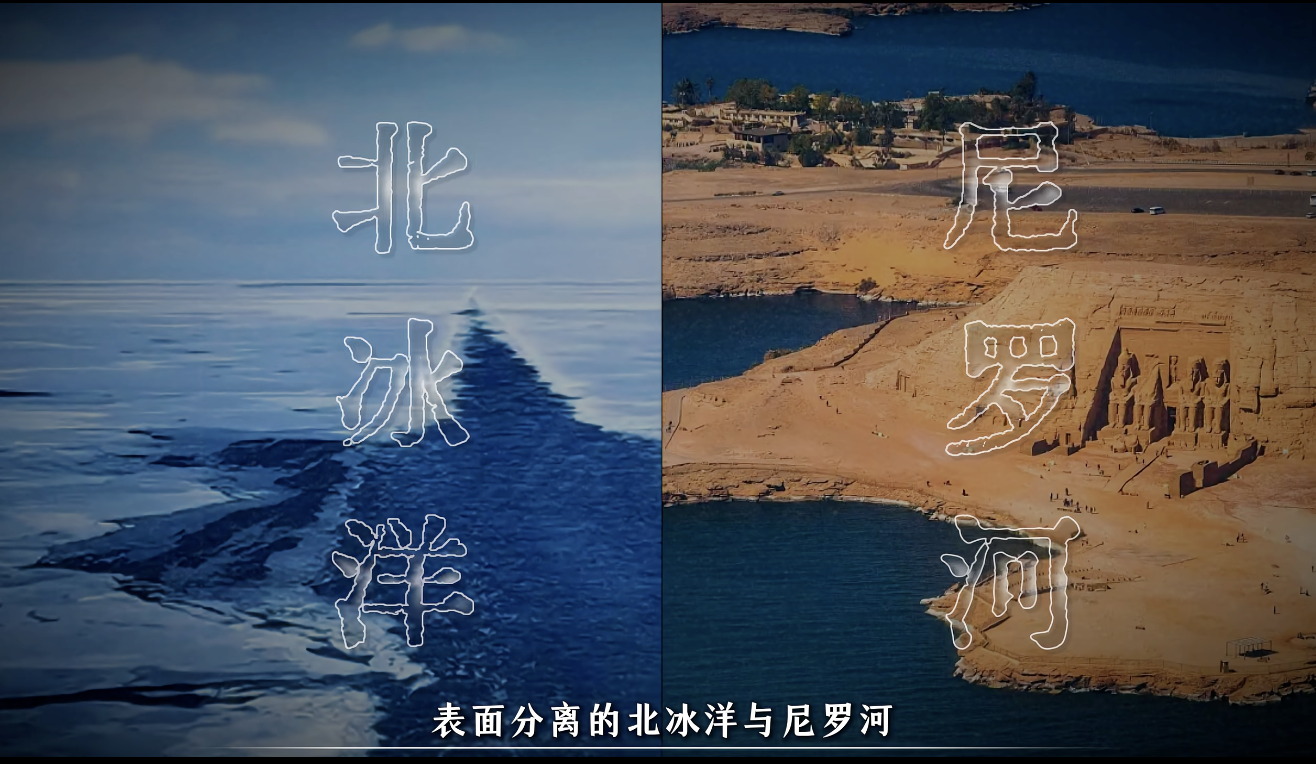
\includegraphics[width=\linewidth]{image/黑塞的水1.png}
        \caption{万物归一示意图}
        \label{fig:water1}
    \end{subfigure}
    \hspace{2em}   % 固定间距，替代 \hfill
    \begin{subfigure}[b]{0.42\textwidth}
        \centering
        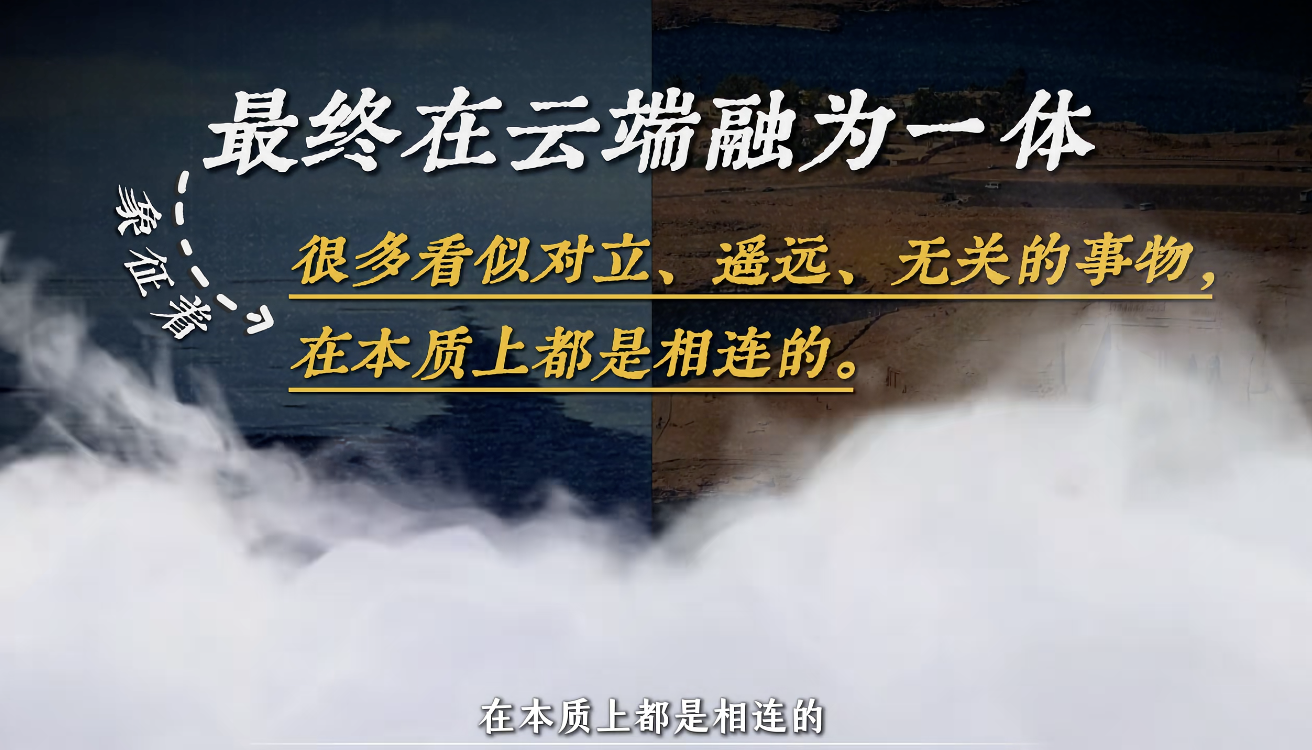
\includegraphics[width=\linewidth]{image/黑塞的水2.png}
        \caption{循环往复示意图}
        \label{fig:water2}
    \end{subfigure}
    \caption{水的哲学意象}
    \label{fig:waters}
\end{figure}


\section{第一组：成长感悟类——引用黑塞名言的写作思路}

\noindent \textbf{通用策略：} 将“水”作为贯穿全文的核心意象（雨、溪流、海、云、眼泪等），在关键转折处点明“水”与“重逢”的关系，结尾直接化用或引用黑塞原句。



\subsection{一、《那一刻，我读懂了\_\_》}

\textbf{题目解读：} 强调从“不懂”到“懂”的瞬间顿悟。适合写亲情、友情、师长教诲、艺术欣赏、自然启示等。

\textbf{引用思路：}
\begin{itemize}
    \item 将“读懂”视为水的“交汇”——曾互不相解，在特殊时刻两条河流在湿云中交融。
    \item 将“那一刻”比作水循环的“蒸发—凝结”节点——困惑升腾为顿悟，再落回清澈。
\end{itemize}

\textbf{写作提纲：}
\begin{enumerate}
    \item \textbf{开头：} 以水的意象引出“不解”，如“我曾以为我和父亲就像两条永不交汇的河。”
    \item \textbf{主体：} 描述“不懂”的日常，然后描写“那一刻”的具体事件，融入雨、泪、汗等水元素。
    \item \textbf{转折：} 瞬间“读懂”，悟到对方的沉默也是另一种流淌。
    \item \textbf{结尾：} “如今我相信，北冰洋与尼罗河会在湿云中交融，而我和父亲，也终于在那一刻读懂了彼此的流向。”
\end{enumerate}

\textbf{示例结尾：}“那一刻，窗外的雨滴连成线，我的泪水也滑落。原来不是所有的爱都要喧哗，有些深流藏在水面之下。就像黑塞说的，北冰洋与尼罗河会在湿云中交融，而我与父亲，也终于在那一刻，读懂了彼此沉默的河床。”



\subsection{二、《这样的挫折让我成长》}

\textbf{题目解读：}强调挫折与成长的因果，需写出具体挫折、内心挣扎和最终收获。

\textbf{引用思路：}
\begin{itemize}
    \item 挫折比作水流的迂回或坠落，但不会停止，最终流向大海。
    \item 成长视为循环——低谷蕴含上升的种子。
    \item 殊途同归——所有弯路终将指向真实自我。
\end{itemize}

\textbf{写作提纲：}
\begin{enumerate}
    \item \textbf{开头：} “我曾以为人生应如直下的瀑布，直到我跌入暗流。”
    \item \textbf{主体：} 叙述一次具体挫折（考试、比赛、人际等），融入汗水、泪水、暴雨等水意象。
    \item \textbf{转折：} 在挫折中找到方法，意识到这是“转弯”而非终点。
    \item \textbf{结尾：} “北冰洋的冰不是结束，是它奔赴尼罗河的前奏。所有的挫折都像水流的低洼，为了在更高的云端与成功重逢。”
\end{enumerate}

\textbf{示例结尾：}“那次失利后，我曾以为我的河流彻底干涸。但时间告诉我，水从未消失，它只是渗入地下，去往另一片海。正如黑塞所写，全世界的水都会重逢，失败与成功也会在生命的云图中交融。这样的挫折，原来是为了让我成长得更深、更阔。”


\subsection*{三、《藏在\_\_里的蜕变》}

\textbf{题目解读：}强调变化发生于隐秘之处、经过时间的酝酿，适合写内在品质、技艺或情感成熟。

\textbf{引用思路：}
\begin{itemize}
    \item 蜕变比作水循环的形态变化——水“藏”入天空，看不见，但最终以雨降落，焕然一新。
    \item “藏”的过程比作地下暗流，默默滋养。
    \item 殊途同归——蜕变前的迷茫和积累，终将汇入更阔的生命之海。
\end{itemize}

\textbf{写作提纲：}
\begin{enumerate}
    \item \textbf{开头：} “我曾以为那些灰暗的练习时光一文不值，它们只是藏在角落里。可后来我才明白，那里正进行着一场水的蜕变。”
    \item \textbf{主体：} 描写“藏”的阶段——重复、枯燥、孤独的努力，细节扎实，隐喻为水在地下渗透。
    \item \textbf{转折：} 默默积累突然显现成果（登台、发表等），蜕变完成，如一滴水升腾成云被阳光照亮。
    \item \textbf{结尾：} “原来，每一滴水的旅程都不是徒劳。藏在暗处的水汽，终将在湿云中与万千水滴相聚，化作彩虹。”
\end{enumerate}

\textbf{示例结尾：}“那些藏在深夜里的反复演练，那些不为旁人所知的咬牙坚持，都像是水在暗处的蒸腾。没有人看到它们，但它们确确实实地上升、汇聚。直到某天，云开雨落，全世界的水都重逢——原来我的蜕变，也是一场北冰洋与尼罗河的遥远合谋。”


\subsection*{四、《为了心中的那束光》}

\textbf{题目解读：}“那束光”象征目标、理想、信念或重要的人，需突出追求过程中的困难与执着。

\textbf{引用思路：}
\begin{itemize}
    \item 将“光”与“水”融合——追求者如朝光蒸腾的水，最终在光中化为云霞。
    \item 循环往复诠释坚持——每一次向光靠近都可能遇到暗礁，但水相信终将与光重逢。
    \item 万物归一——所有努力终将指向那束光，如不同河流归于大海。
\end{itemize}

\textbf{写作提纲：}
\begin{enumerate}
    \item \textbf{开头：} 直接点明“光”，并用水的意象引入：“我是一滴水，心中却藏着一片海洋，而那片海洋的名字，就是远方的那束光。”
    \item \textbf{主体：} 叙述追寻光的过程中的困难、诱惑、犹豫，穿插汗、雨、泪等水元素。
    \item \textbf{转折：} 低谷时，光依然在远方或突然变亮，激励前行。
    \item \textbf{结尾：} “我相信，只要不放弃流动，每一滴水都能抵达光的怀抱。北冰洋与尼罗河在湿云中交融，而我心中的那束光，也终将与我所有的汗水、泪水在云端相拥。”
\end{enumerate}

\textbf{示例结尾：}“为了那束光，我流过干旱的沙漠，也经过严寒的冰原。但我记得黑塞的话——全世界的水都会重逢。光与水本就是一体，当我终于蒸腾成云，那束光穿透我的身体，我便成了朝霞。原来，为了心中的那束光而奔跑，就是让一滴水找到自己的星空。”


\section{通用化用要点}
\begin{tcolorbox}[colback=yellow!10, colframe=orange!50, title=化用要点]
\begin{enumerate}[leftmargin=*]
    \item \textbf{铺垫要自然：} 前文至少出现一次与“水”相关的意象（雨、海、汗、泪、溪流等），使结尾的名言不突兀。
    \item \textbf{不必全句照搬：} 可拆解为“北冰洋的寒流”“尼罗河的暖”“湿云”“重逢”等碎片，穿插在叙事中。
    \item \textbf{避免说教：} 哲理要通过故事本身渗透，而不是直接喊口号。
    \item \textbf{保持真诚：} 所写事件必须真实或可信，否则名言的厚重感会被削弱。
\end{enumerate}
\end{tcolorbox}


\section{坚持}


坚持开头:“不积跬步无以至千里，不积小流无以成江海”没有一蹴而就的胜利，只有厚积薄发的坚持。坚持不一定能成功，但坚持能够让我们对生命和未来仍有所期待。

结尾：“古之成大事者不惟有超世之才，亦必有坚韧不拔之志”平坦的康庄大道，不需要坚持。崎岖的蜿蜒小路，才是命运对你的考验。再坚持一下，是一种信念，也是一种转机。


\section{幸好有苏试}


\begin{tcolorbox}[colback=blue!5, colframe=blue!50, title=主题一：旷达乐观的处世哲学]
适用场景：面对人生风雨、逆境与挑战时的态度。
素材支撑：乌台诗案后被贬黄州，苏轼并未沉沦。他脱下长衫开荒种地，自号“东坡居士”；买不起羊肉便发明“东坡肉”；雨中穿林打叶，依然能吟出“一蓑烟雨任平生”。 他的乐观是将绝境活成生活美学。
\end{tcolorbox}

\begin{tcolorbox}[colback=green!5, colframe=green!50, title=主题二：坚韧不拔的生命韧性]
适用场景：讨论坚持、生命力、在困苦中成长。
素材支撑：晚年被贬至当时被视为绝境的海南儋州，60多岁的苏轼没有等死，而是 在当地办起学堂亲自讲学，培养出海南历史上第一位举人 。他将个人苦难转化为泽被苍生的行动。
\end{tcolorbox}

\begin{tcolorbox}[colback=orange!5, colframe=orange!50, title=主题三：破茧成蝶的思想格局]
适用场景：谈格局、放下个人恩怨、精神境界。
素材支撑：苏轼能跳出二元对立的局限。最典型的是，他虽与王安石政见不合，但在王安石罢相后主动拜访，两人同游中山、谈诗论道， 留下“相逢一笑泯恩仇”的佳话 。
\end{tcolorbox}


\subsection{幸好有苏轼}

文字，是两个灵瑰交流最直接的方式。
——题记

又是一个"不眠之夜"！
望着铺天盖地的试卷，透过窗户的反光，我看到一个憔悴的自己。压力如石的初三，盲目努力而未得回报，我身处黑暗，内心充满绝望和不甘。
我打开窗户，清冷的风灌了进来，我又随手打开了摘抄本。

"竹杖芒鞋轻胜马，谁怕？一蓑烟雨任平生"映入眼帘，我被这些文字吸引，进入了苏轼的时空。

寒风仍在吹，有雨，还有一个吟咏长啸、悠然自得的诗人，即使是竹杖芒鞋行走在泥泞之中也毫不在意，反而仰面朝天，任凭雨点打落，他是那么从容不迫，眼角有笑意，眼中有深意。"归去，也无风雨;也无晴"，他豁达大度，我疑惑，明明有风雨，为何他却说"也无风雨也无睛"？还没缓过神来，他继续说道："人生几时欢喜几时愁，雨后仍是晴空，我东坡的一生，有得意有坎坷，归来，心中仍怀大志！"
寒风又灌了进来，回过神，我想起苏轼在《自题金山画像》中写到的那甸"问汝平生功业，黄州惠州儋州"，虽有自嘲的意味，但也写出了贬谪生涯在他一生中的重要位置。也许正是仕途中的低谷，成就了他思想、性格、心态上的乐观豁达，乃至文学上的高峰。那我今天的低谷又算得了什么呢？我释然一笑，打开了那份沉重的成绩单，"人有悲欢离合，月有阴晴圆缺"，只要我心向阳，又怎会怕眼前短暂的黑暗呢？

目光又被另一句诗吸引："粗缯大布裹生涯，腹有诗书气自华。"一个身着布衣、朴实无华的诗人再次出现在我眼前，他手握诗卷，望向远方，他领悟人生于心中，寄托情怀于诗书里。

我如梦初醒，幸好有苏轼。他引导我走出黑暗，他引导我在乐观向上的人生道路上前行，他引导我在文字中领悟诗意之美。

、幸好有苏轼。我在摘抄本上写下：无论雨，无论睛，腹有诗书，文笔留韵。
这，无疑是一场我与东坡通过文字进行的灵魂交流。——后记


\chapter{写作XX}


\section{写作（50分）}

阅读下面的文字，根据要求写作。（50分）

并非站在山顶，才能被看见。

以上文字引发了怎样的联想和思考？请联系自己的生活经历和感受，写一篇文章。


凡人微光

\chapter{考场练兵答案}

\section{选择}

\paragraph{1.} 答案：C

解析：A. 语序不当，改为：既影响了汉语表意功能的发挥，也消解了中国文化精深而丰富的内涵；B. 两面对一面，去掉“能否”或在“在于”后加上“能否”；D. 关联词语使用不当，改“尽管”为“不管”。

% 第2题
\paragraph{2.} 答案：B

解析：B. 成分残缺，应在“环境保护”后加上“力度”。

% 第3题
\paragraph{3.} 答案：B

解析：B. 搭配不当。“效率”与“改动”“改变”都不能搭配，应将“改动”改为“提高”。

% 第4题
\paragraph{4.} 答案：C

解析：C. “该句有语病，应把‘提升’改为‘提高’”有误，“提升了民族文化的交流”搭配不当，应把“提升”改为“促进”。

% 第5题
\paragraph{5.} 答案：B

解析：A. 语序不当，将“我们”放在“只有”前；C. 否定不当，删去“不再”；D. 搭配不当，将“表示”改为“表达”。


\section{阅读}

\begin{enumerate}[leftmargin=*]
    \item （1）fēng ráo \quad （2）污秽
    \item （3）C \quad （4）A \quad （5）B
    \item B
    \item 夜夜我听见马蹄奔驰的声音，草原的儿子在黎明的天边呼唤。
\end{enumerate}

解析：

\subsection*{（1）}
\begin{itemize}[leftmargin=*]
    \item 丰饶（fēng ráo）：丰裕富饶；丰足充实。
    \item 污秽（wū huì）：肮脏的；不洁净的（物体）。
\end{itemize}

\subsection*{（2）}
\begin{itemize}[leftmargin=*]
    \item 谦逊：谦虚、不浮夸，不自大或不虚夸。
    \item 宽广：面积大，宽阔。
    \item 坚韧：指物体坚固而柔韧，不容易折断；指人的性格品质不屈不挠，意志坚定，坚忍有韧性。
\end{itemize}

第一空：在此形容意志，应用“坚韧”，故选 C。\\
第二空：在此形容气质，应用“谦逊”，故选 A。\\
第三空：在此形容胸怀，应用“宽广”，故选 B。

\subsection*{（3）}
本题考查词性。

B.“他们看来是很平凡、很简单的哩”中的“很”是副词；故选 B。

\subsection*{（4）}
本题考查病句修改。

“看见”与“声音”搭配不当，应将“看见”改为“听见”。